\chapter{\color{Millum}\textbf{Diskusjon}}
I dette avsluttende kapittelet skal vi diskutere utfordringer, drøfte valg som er gjort og vurdere vår innsats i prosjektet.

\section{\textbf{Tekniske utfordringer}} \label{Tekniske_utfordringer}

Alle utviklingsprosjekter byr på utfordringer. I avsnittene \textbf{\ref{Tekniske_utfordringer}} og \textbf{\ref{Andre_utfordringer}} skal vi ta en titt på de tekniske og menneskelige utfordringene vi opplevde, og hvordan vi håndterte disse. 

\subsubsection{\textbf{Håndtering av desimaltall}}

Millum sine kunder er stort sett basert i Skandinavia og vi har derfor vært nødt til å støtte flere språk i applikasjonen vår. I Norge og flere andre land brukes komma som desimalskille, mens andre land bruker for eksempel punktum ved håndtering av desimaltall. Når det gjelder håndtering av desimaltall har vi støtt på en utfordring som spiste mye mer arbeidstid enn forventet. 

Under en varetelling som vist tidligere \ref{fig:DesignInputStepper} gir vi bruker mulighet til å telle en vare med et inntastingsfelt \textit{eller} ved å trykke på pluss eller minus.

Et eksempel på å legge inn et inntastingsfelt med HTML
\begin{lstlisting}
<input type="number">
\end{lstlisting}

Standarden til Typescript når man har et inputfelt med tallverdier er at desimalskillet er punktum, og ikke godtar komma. Vi måtte derfor bruke inputfelt med tekstverdier for å tillate dette. Dette skapte videre problemer fordi ugyldige verdier som bokstaver, tegn og lignende kan bli fylt inn. Det er \textit{kun} tall som er gjeldende for inntastningsfeltet og for at det skal bli håndert riktig av applikasjonen må vi sørge for at bruker ikke kan skrive inn ugyldige tegn. I tillegg  vil det numeriske tastaturet på mobilen ikke vises på grunn av input-typen ``tekst``. 

Vi kom derfor frem til denne fremgangsmåten for å løse problemene

\begin{enumerate}
    \item \textbf{Fjerne ugyldige verdier.} Herunder alle bokstaver, spesialtegn, overflødige nuller og duplikater av skilletegn ved bruk av regulære utrykk og konvertere fra tekst til tall.
    
    \begin{figure}[H] 
        \centering
        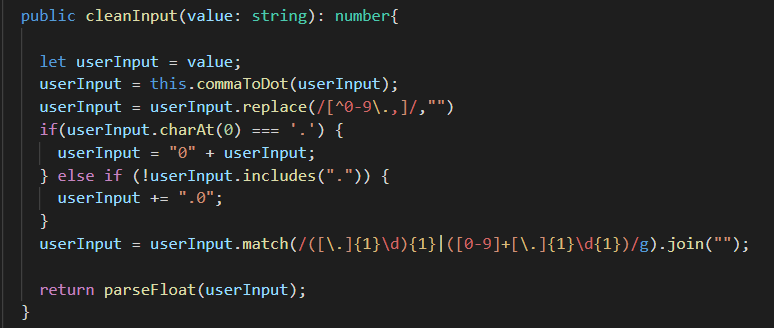
\includegraphics[width=120mm]{figures/Utfordringer/cleanInput.PNG}
        \caption{Bruk av regulære utrykk for å fjerne ugyldige verdier.}
    \end{figure}
    
    \item \textbf{Konvertere skilletegn} basert på brukerens språk ved å hente opp valgt språk, og sjekke hvilken standard for desimaltegn blir brukt.
    
    \begin{figure}[H] 
        \centering
        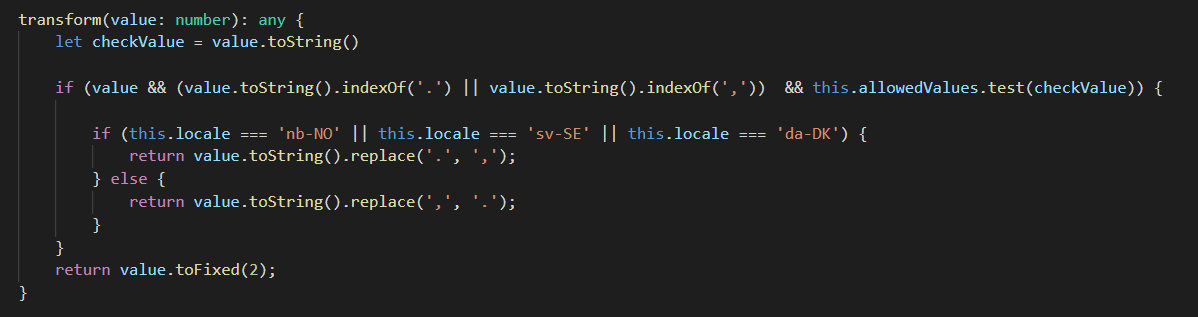
\includegraphics[width=120mm]{figures/Utfordringer/numericFormat.PNG}
        \caption{Kodesnutt av numericFormat-pipe.}
    \end{figure}
    
    \item \textbf{Tvinge keyboard til å kun vise tall} ved å sette input-modus til ''numeric''.
    
    \begin{figure}[H] 
        \centering
        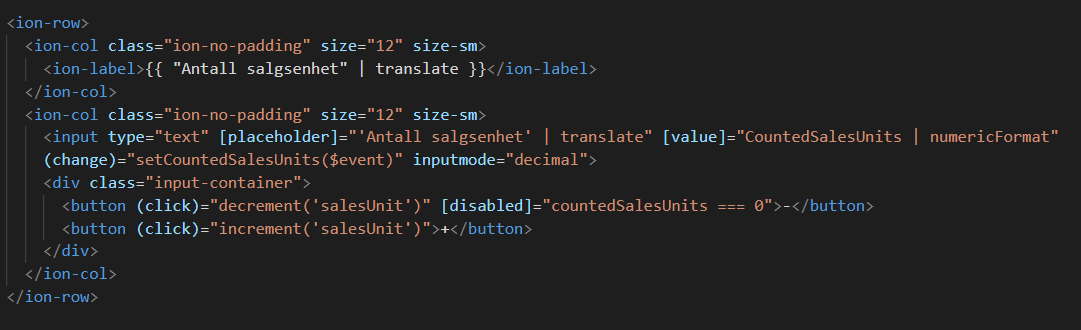
\includegraphics[width=120mm]{figures/Utfordringer/stock-taking-count-codeSnippet.PNG}
        \caption{Kodesnutt av et inntastningsfelt under en varetelling.}
    \end{figure}
    
\end{enumerate}


Med de tre punktene ovenfor har vi klart å eliminere hovedutfordringen ved å fremvise desimaltall basert på hvilket språk brukeren har. Dette var en user story vi opprinnelig hadde estimert rundt én arbeidsdag til å gjennomføre, men ettersom dette var en utfordring ingen av oss hadde støtt på tidligere gikk det nærmere en halv sprint med diskusjon og testing. Sluttresultatet oppfyller atferden inntastingsfeltene bør og må ha. I tillegg fikk vi virkelig oppleve det å feilestimere tid under en ''task'' i Scrum-rammeverket.

%% Referer til vurdering av scrum og hvordan feilestimeringer påvirker måten man jobber på



\section{\textbf{Andre utfordinger}} \label{Andre_utfordringer}

I sammenheng med virusutbruddet av Covid-19 gikk oppdragsgiver den 19. Mars ut med permitteringsvarsler for samtlige ansatte i organisasjonen. Avdelingslederen var rask på banen til å følge opp oss for å sørge for at vi fortsatt kunne gjennomføre hovedoppgaven vår i så høy grad det var mulig. Dessverre hadde dette uventede konsekvenser for oss. Vi hadde blant annet ikke lenger mulighet til å gjennomføre planlagte brukertester med kunder, og vi ble nødt til å skrinlegge noe planlagt funksjonalitet. Siden utviklingsmiljøet til oppdragsgiveren var lukket var vi nødt til å få på plass VPN (Virtual Private Network. Brukes til å koble seg på lukket nett utenifra). Dessverre var det ikke mulig å koble seg på VPN på mobiltelefon som ga oss utfordringer med å jobbe hjemmefra. Til tross for dette hadde vi allerede kommet langt på løsningen og var tilpasningsdyktige i denne turbulente tiden. Det er i slike situasjoner man reflekterer over hvor viktig en god prosess er, så man alltid har mulighet til å tilpasse seg nye situasjoner.

Som en følge av permitteringssituasjonen hos oppdragsgiver hadde vi heller ikke mulighet til å teste applikasjonen i produksjonsmiljøer, og vi måtte derfor definere leveransekravet på nytt ettersom vi ikke kan lansere en applikasjon som ikke er testet med reel data. Selv om dette ikke var problematisk for vår del skulle vi gjerne ha fulgt hele løpet fra innsiktfasen til produksjonssetting som vi opprinnelig hadde planlagt. Vi kommer tilbake til vurdering av situasjonen i 

\section{\textbf{Vurdering av arbeidsmetodikk}} \label{Vurdering_SCRUM}
\newthought{Å bruke en variant av SCRUM} som arbeidsmetodikk har vært til stor hjelp for oss underveis i prosjektet. Siden man kan bruke SCRUM som et rammeverk og velge eller luke bort deler av metodikken kan man skreddersy arbeidsmetodikk som passer teamet. I vårt tilfelle har det å kunne inkludere oppdragsgiver underveis i prosessen via sprintpresentasjoner vært svært viktig, mens daglig standup kanskje ikke alltid har vært like viktig siden vi har jobbet så tett store deler av prosjektet. Muligheten til å raskt omstille seg til nye situasjoner er kanskje bærebjelken til smidig metodikk og som vi nevnte i (\textbf{\ref{Andre_utfordringer}}) fikk vi smake dette på alvor i situasjonen som utspilte seg i forbindelse med virusutbruddet av Covid-19. 

Samtidig medfører en slik arbeidsmetodikk ekstra møter og tid i forbindelse med planlegging, presentasjoner og lignende. En utfordring med dette er kanskje motivasjonen til å være forberedt og gjennomføre disse møtene. Det har derfor vært viktig for gruppen å kommunisere på en god måte slik at arbeidsmoralen forble høy. 

\section{\textbf{Vurdering av forankring i forskning}}
Vi har i prosjektets løpetid benyttet oss av litteratur knyttet til systemarkitektur og design/brukeropplevelse. Det har vært viktig for oss å gjøre designvalg som er basert på forskning og har derfor brukt forskning gjort av Nielsen Norman Group og litteraturen til William Lidwell (2003).

For gjennomføring av spørreundersøkelser har vi støttet oss på litteraturen til Oates (2006). Vi hadde lite erfaring med datainnsamling og hadde høyt læringsutbytte i forbindelse med gjennomføring av emnet ``Undersøkelsesmetoder`` og litteraturen til Oates. Til tross for dette ser vi i ettertid at vi burde forsøkt å benytte flere datainnsamlingsmetoder for å kvalitetssikre og forsterke den eksisterende forskningen.

Både vi og oppdragsgiver var opptatt av å designe systemarkitekturen etter kjente metoder og prinsipper. Vi støttet oss derfor på litteraturen til C. Martin (2001). Kodebasen kan ganske raskt bli uoversiktlig og uleselig dersom man ikke tydelig følger prinsippene. Vi er fornøyd med sluttresultatet til arkitekturen i applikasjonen.

\section{\textbf{Vurdering og diskusjon av løsningen}}

\subsection{\textbf{Verktøy og rammeverk}}

Ved oppstart av prosjektet hadde vi flere veier vi kunne gå, og vi endte opp med å bruke de teknologiene Millum selv tar i bruk. For noen av oss på gruppen innebar dette teknologier vi hadde god erfaring med, og noen teknologier vi hadde mindre erfaringer med. I løpet av prosjektet så vi klart at vi ble langt mer bekvemme med teknologiene vi hadde mindre erfaringer med.

I underpunktene vil vi presentere de tekniske verktøy og rammeverk vi har jobbet med og vår vurdering av disse.


\begin{itemize}
    \item \textbf{Ionic}
        %\newline Ionic har fungert utmerket som kryssplattformsløsning for oss. Vi har hatt spesielt få problemer med å kjøre og teste løsningen på mobilenhetene vi har hatt til rådighet. Det vi har å utsette på er ikke selve teknologien, men dokumentasjonen. Selv om dokumentasjonen til Ionic er omfattende har vi stått på hindre ved å ta i bruk deres komponenter som krever mer logikk.%
        
        Ionic har gitt oss mulighet til å utvikle mot flere plattformer med samme kodebase, dette har vært svært verdifullt for prosjektet vårt, men også for oppdragsgiver når de videre skal utvikle og supportere applikasjonen. En av utfordringene vi sto ovenfor var i forbindelse med kompilering og testing mot mobilenhetene. Dette kunne ta flere minutter per endring, så enkelte problemer kunne ta svært lang tid å løse. Til tross for dette er vi på generelt grunnlag veldig fornøyd med måten vi brukte Ionic, og hvordan det hjalp oss å utvikle løsningen.
        
    \item \textbf{Angular}
        \newline 
        
    \item \textbf{TypeScript}
        %\newline Alle på gruppene hadde tidligere erfaring med TypeScript på forskjellige nivåer. Det å kode i TypeScript er en stor forbedring i motsetning til å skrive alt i JavaScript med tanke på at man kan velge, og oftest, skriver kode mer eksplisitt. Dette er på grunn av type inferens, noe vi har vært utrolig takknemlig for. Når vi da transpilere kode vil vi fort klare å luke ut feil. Som med alle nye programmeringsspråk man ikke har like god erfaring med vil det alltid gå ekstra tid til å bli komfortable. Dette er en kostnad som er aboslutt verdt det, spesielt når vi så at prosjektet begynte å vokse i størrelse.%
        
        Til sammenligning med tradisjonell JavaScript lar TypeScript deg skrive sterke typer, det vil si eksplisitte datatyper som number (tall), string (tekst) m.m. Fordelen med dette er at vi kan være sikre på at dataene vi sender til API-ene ikke er søppeldata, og at API-et i større grad vi håndtere kommunikasjonen bedre. I tillegg så må TypeScript kompileres for å kjøres, i motsetning til tradisjonell JavaScript. Dette gjør at man kan få feilmeldinger før man i det hele tatt tester koden i applikasjonen, og kan luke ut feil tidlig i utviklingen. På en annen side krevde det en del innsats og tid for å bli godt kjent med TypeScript, for de som ikke hadde like mye erfaring med det. 
        
        
    \item \textbf{Team Foundation Server}
        \newline TFS var ukjent for to av medlemmene, og vi fikk en kort opplæring av Andreas. Å bruke TFS ga oss mulighet til å ha en samlet plattform som inneholdt mange verktøy vi brukte i prosessen som:
        \begin{itemize}
            \item Task board for å organisere
            \item Gitverktøy
            \item Pull Request
            \item m.m
        \end{itemize}
        I tillegg til at oppdragsgiver hadde mulighet til å følge med på utviklingen, konkret svare på spørsmål knyttet til oppgaver og lignende. Selv om vi er fornøyd med hvordan TFS har fungert for gruppen vår hadde det kanskje vært tilstrekkelig å bruke et kanban-board og eksempelvis Github til å være vert for kildekoden.  
    
    
\end{itemize}

\section{\textbf{Vurdering av ambisjonsmål}}
Som nevnt i \textbf{\ref{Ambisjoner}} hadde vi i starten av prosjektet satt opp en liste med ambisjonsmål for hovedoppgaven vår. Disse rangerte vi fra viktigst til minst viktig. I dette avsnittet drøfter vi målene vi satt.

\begin{description}
    \item{\textbf{Utvikle en løsning som reduserer tid og kostnad ved gjennomføring av varetellinger. }}
    Å utvikle en løsning som er i tråd med vårt mål om å redusere tid og kostnad i forbindelse med varetellinger oppleves for oss som nyttig, noe som bekreftes av tilbakemeldingene fra oppdragsgiver og kunder som har testet løsningen vært svært positive. Til tross for dette skulle vi gjerne ha gjennomført flere undersøkelser for å kartlegge tid- og kostnadbruk i forkant og etterkant av lanseringen til løsningen.
    
    \item{\textbf{Levere en god akademisk oppgave}}
    Selv om alle oppgaver, inkludert denne har forbedringspotensiale så har det å kunne levere en så stor oppgave gitt oss et stort læringsutbytte. Det å vite at denne rapporten er det siste vi skal levere i forbindelse med bachelorstudiet har motivert oss til å skrive det vi mener er en god akademisk oppgave. 
       
    \item{\textbf{Få erfaring}}
    Denne reisen har gitt oss mulighet til å gjennomføre et prosjekt fra innsikt- og analyse til leveranse av et ferdig produkt. Det er svært givende å ha vært gjennom, og samtlige gruppemedlemmer kunne ikke vært foruten denne gode erfaringen og kommer til å dra nytte av den i karrieren vår.
    
    \item{\textbf{Personlig utvikling}}
    Når man er en så liten gruppe mennesker som skal levere en ferdig mobilapplikasjon samtidig som man skriver hovedoppgaven sin er det ingen tvil om at man må ta på seg mange hatter. Ingen er best i alt, men her har alle fått utfordret seg selv og egne evner. Det gjør oss rustet til å tørre å ta sjanser og prøve nye ting, enten det er å begynne på mastergrad, jobbe med utviklingsprosjekt eller noe i mellom. 
    
\end{description}

\section{\textbf{Konklusjon}}


